\documentclass[tikz, border=10pt]{standalone}
\usetikzlibrary{shapes.geometric, arrows.meta, positioning, fit, calc}

\begin{document}
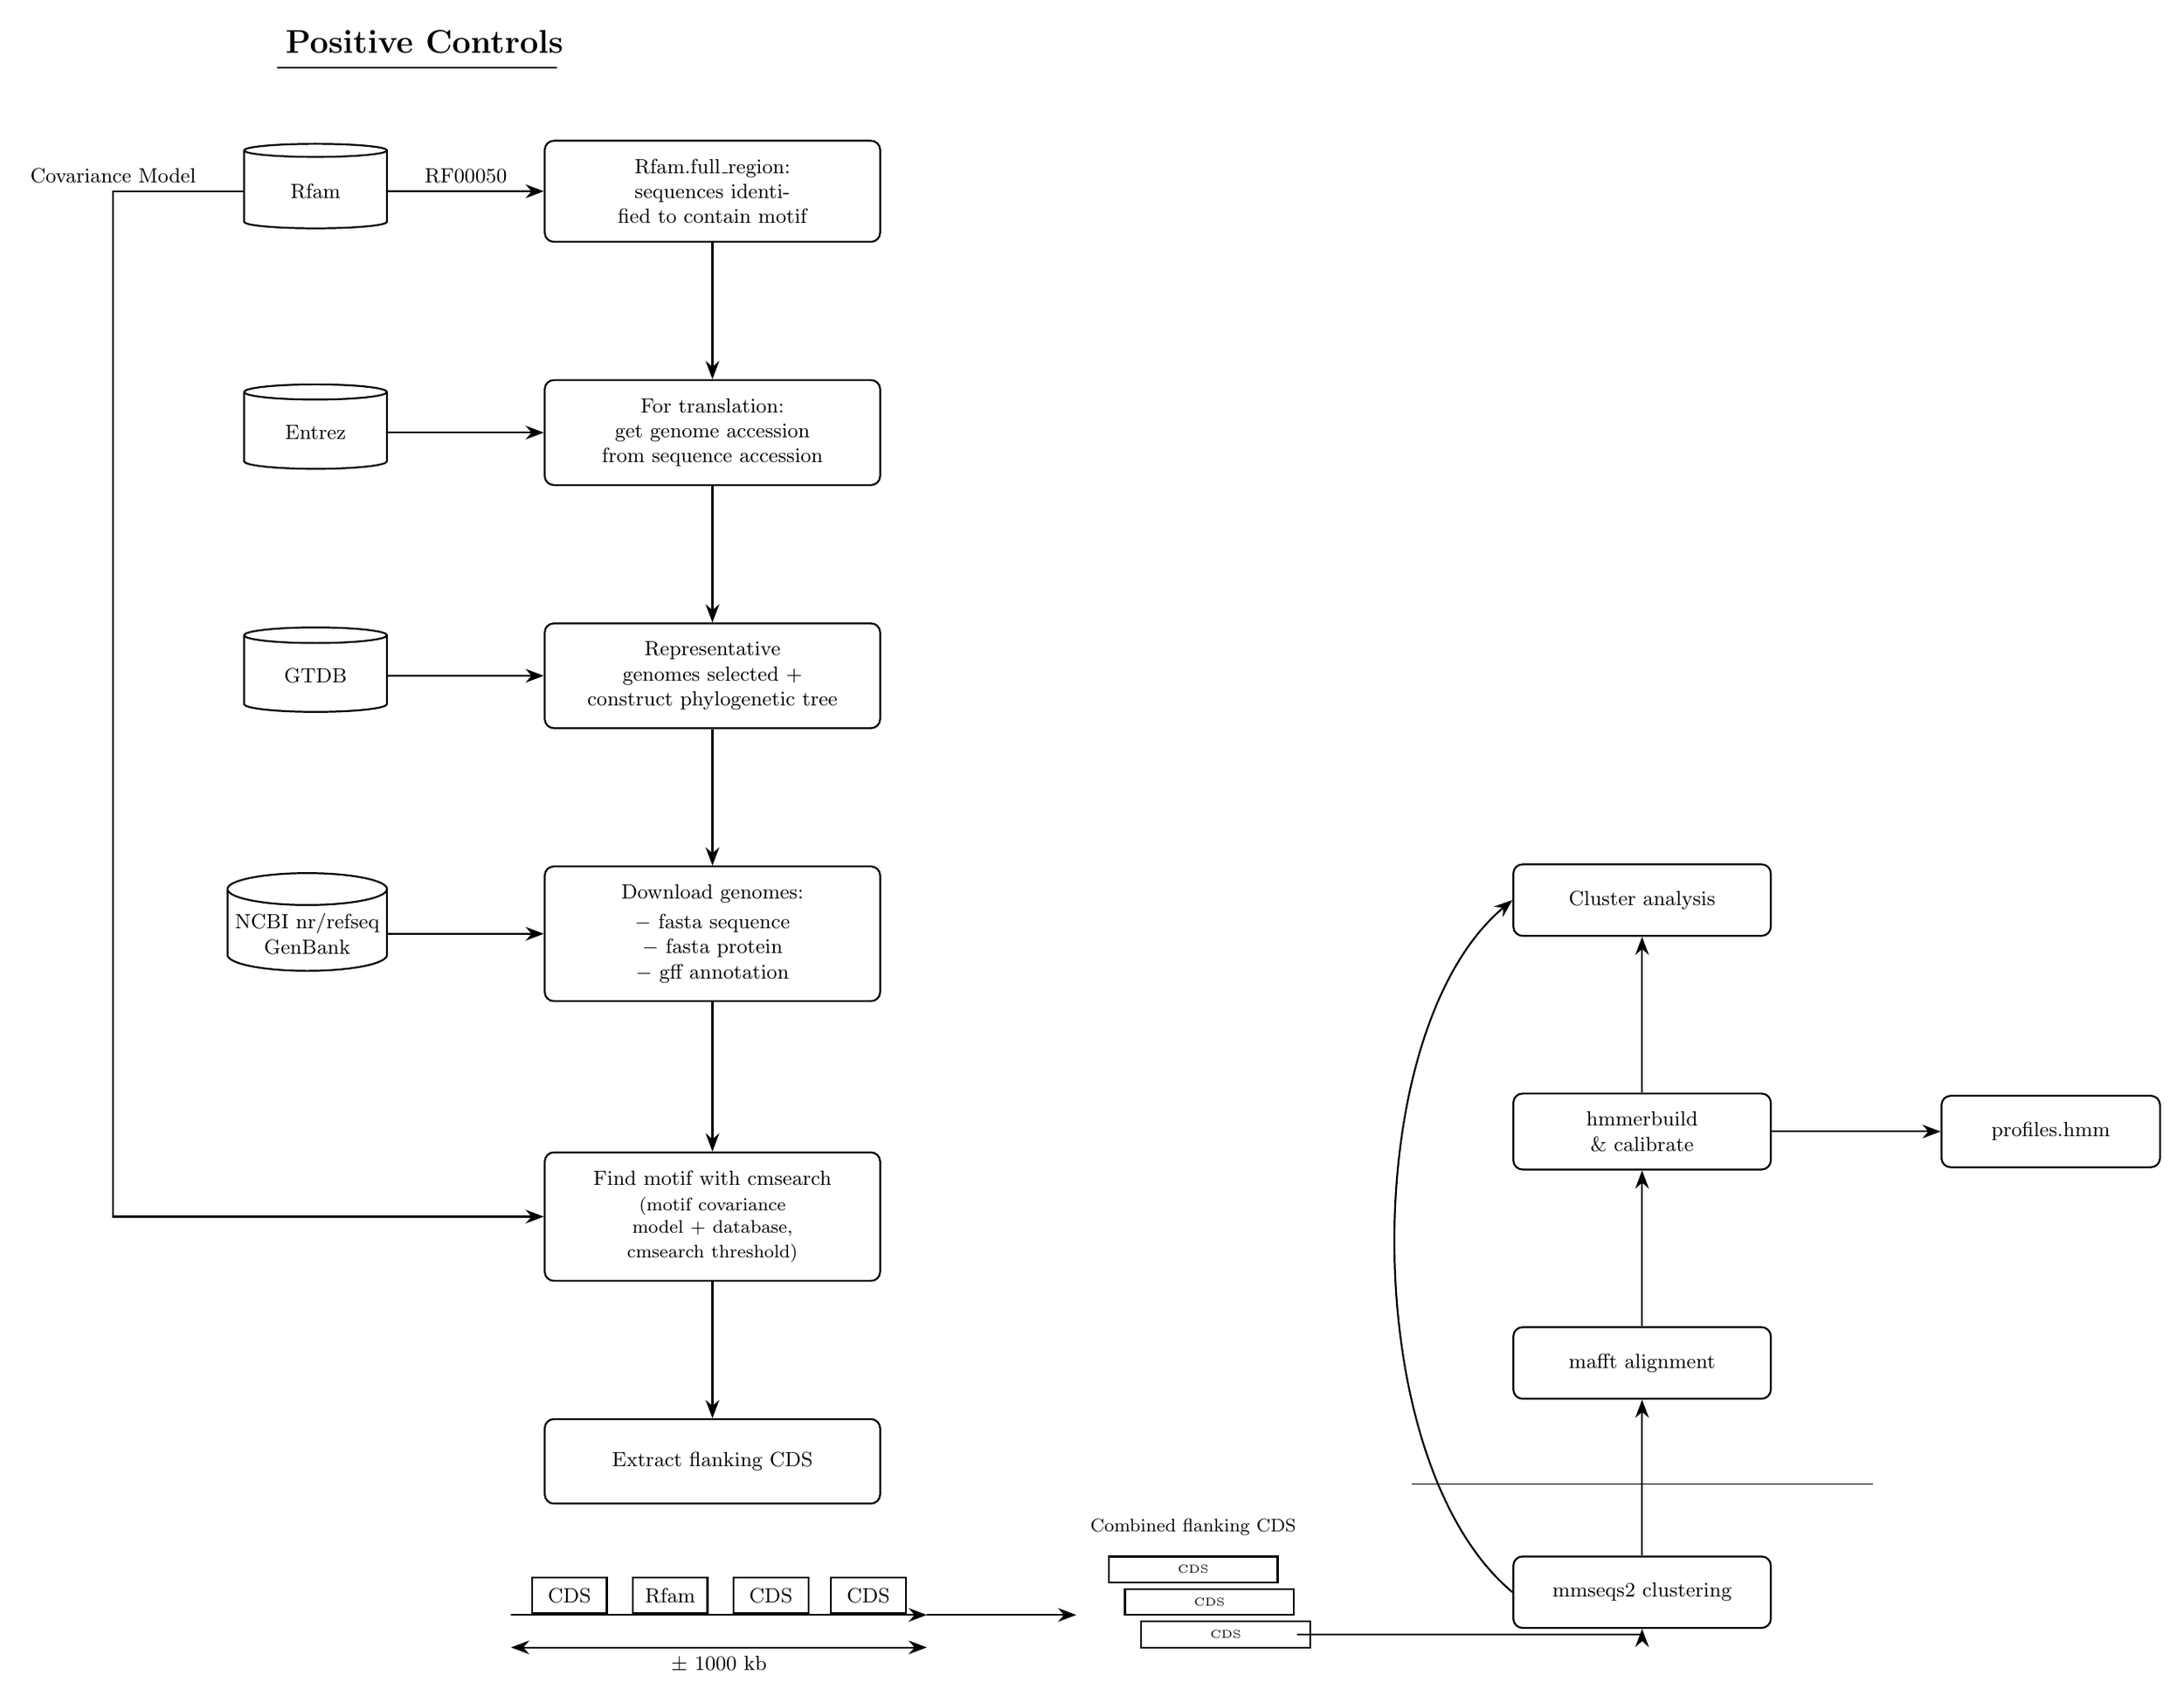
\begin{tikzpicture}[
    font=\small,
    db/.style={cylinder, shape border rotate=90, aspect=0.2, draw, thick,
        minimum height=1.3cm, minimum width=2.2cm, align=center},
    proc/.style={rectangle, draw, thick, rounded corners, align=center,
        text width=4.6cm, minimum height=1.3cm, inner sep=8pt},
    proc2/.style={rectangle, draw, thick, rounded corners, align=center,
        text width=3.4cm, minimum height=1.1cm, inner sep=8pt},
    gene/.style={rectangle, draw, thick, minimum height=0.55cm},
    >={Stealth[length=2.8mm]},
    every path/.style={thick},
    node distance=1.6cm and 2.4cm,
]

% ============ Title ============
\node[font=\Large\bfseries, anchor=west] at (-1.7,11.3) {Positive Controls};
\draw (-1.7,10.9) -- (2.6,10.9);

% ============ Main vertical pipeline ============
\node[proc] (fullregion) at (5,9)
    {Rfam.full\_region:\\sequences identified to contain motif};
\node[db, left=of fullregion] (rfam) {Rfam};
\draw[->] (rfam) -- node[above]{RF00050} (fullregion);

\node[proc] (translate) [below=2.1cm of fullregion]
    {For translation:\\get genome accession from sequence accession};
\node[db, left=of translate] (entrez) {Entrez};
\draw[->] (fullregion) -- (translate);
\draw[->] (entrez) -- (translate);

\node[proc] (repgenomes) [below=2.1cm of translate]
    {Representative genomes selected +\\construct phylogenetic tree};
\node[db, left=of repgenomes] (gtdb) {GTDB};
\draw[->] (translate) -- (repgenomes);
\draw[->] (gtdb) -- (repgenomes);

\node[proc] (download) [below=2.1cm of repgenomes]
    {Download genomes:\\[2pt]
     $-$ fasta sequence\\
     $-$ fasta protein\\
     $-$ gff annotation};
\node[db, left=of download] (ncbi) {NCBI nr/refseq\\GenBank};
\draw[->] (repgenomes) -- (download);
\draw[->] (ncbi) -- (download);

\node[proc] (cmsearch) [below=2.3cm of download]
    {Find motif with cmsearch\\[2pt]
     \footnotesize (motif covariance model + database,\\cmsearch threshold)};
\draw[->] (download) -- (cmsearch);

% long feed straight down from Rfam supplying the covariance model
\draw[->] (rfam.west) -- ++(-2.0,0) node[above]{Covariance Model} |- (cmsearch.west);

\node[proc] (extract) [below=2.1cm of cmsearch] {Extract flanking CDS};
\draw[->] (cmsearch) -- (extract);

% invisible anchor point where the gene cartoon begins (relative to extract, not hardcoded)
\coordinate (generow) at ($(extract.south)+(-3.1,-1.7)$);
%\draw[->] (extract.south) -- ($(generow)+(3.2,0.3)$);

% gene cartoon: CDS - Rfam - CDS - CDS  (~1000 kb span)
\begin{scope}[shift=(generow)]
    \draw[->] (0,0) -- (6.4,0);
    \node[gene, minimum width=1.15cm] (g1) at (0.9,0.3)  {CDS};
    \node[gene, minimum width=1.15cm] (g2) at (2.45,0.3) {Rfam};
    \node[gene, minimum width=1.15cm] (g3) at (4.0,0.3)  {CDS};
    \node[gene, minimum width=1.15cm] (g4) at (5.5,0.3)  {CDS};
    \draw[<->] (0,-0.5) -- (6.4,-0.5) node[midway, below] {$\pm$ 1000 kb};
\end{scope}

% ============ Right side: clustering / alignment / profile pipeline ============
\coordinate (combinedanchor) at ($(generow)+(9.2,0)$);
\node[align=center, font=\footnotesize] (combined_label) at ($(combinedanchor)+(1.3,1.35)$) {Combined flanking CDS};
\begin{scope}[shift=(combinedanchor)]
    \draw[thick] (0,0.5)   rectangle ++(2.6,0.4) node[pos=.5]{\tiny CDS};
    \draw[thick] (0.25,0)  rectangle ++(2.6,0.4) node[pos=.5]{\tiny CDS};
    \draw[thick] (0.5,-0.5) rectangle ++(2.6,0.4) node[pos=.5]{\tiny CDS};
\end{scope}
\draw[->] ($(generow)+(6.4,0)$) -- ++(0.8,0) |- ($(combinedanchor)+(-0.5,0)$);

\node[proc2] (mmseqs) [right=3.2cm of combined_label, yshift=-1cm] {mmseqs2 clustering};
\draw[->] ($(combinedanchor)+(2.9,-0.3)$) -| (mmseqs.south);

% multiple-alignment block placeholders feeding mmseqs2 (purely decorative, anchored above mmseqs)
\node[font=\tiny] at ($(mmseqs.north)+(-1.6,1.1)$) {\rule{1.3cm}{0.6pt}\\[2pt]\rule{1.3cm}{0.6pt}\\[2pt]\rule{1.3cm}{0.6pt}};
\node[font=\tiny] at ($(mmseqs.north)+(0,1.1)$)    {\rule{1.3cm}{0.6pt}\\[2pt]\rule{1.3cm}{0.6pt}\\[2pt]\rule{1.3cm}{0.6pt}};
\node[font=\tiny] at ($(mmseqs.north)+(1.6,1.1)$)  {\rule{1.3cm}{0.6pt}\\[2pt]\rule{1.3cm}{0.6pt}\\[2pt]\rule{1.3cm}{0.6pt}};

\node[proc2] (mafft) [above=2.4cm of mmseqs] {mafft alignment};
\draw[->] (mmseqs) -- (mafft);

\node[proc2] (hmmbuild) [above=2.4cm of mafft] {hmmerbuild \& calibrate};
\draw[->] (mafft) -- (hmmbuild);

\node[proc2, text width=2.8cm] (profiles) [right=2.6cm of hmmbuild] {profiles.hmm};
\draw[->] (hmmbuild) -- (profiles);

\node[proc2] (clusteranalysis) [above=2.4cm of hmmbuild] {Cluster analysis};
\draw[->] (hmmbuild) -- (clusteranalysis);
\draw[->] (mmseqs.west) .. controls ($(mmseqs.west)+(-2.4,2)$) and ($(clusteranalysis.west)+(-2.4,-2)$) .. (clusteranalysis.west);

\end{tikzpicture}
\end{document}
